\section{Examples}
% Organize this section according to major topics
% give each topic a section heading in boldface.
% try to cover the major common points :
%
% problem design
% methods of measurement
% supporting models
% supporting data
% simulations run
% results

% Just write the section headings for each part and indicate what goes in that
% section with words :
%
% heading
% figures (with captions)
% schematics (with captions and footnotes)
% equations
% tables

% What does it mean?
% What did I actually test?
% What were the results?
% Did the work yield a new method?
% Did the work yield new knowledge?
% What measurements did I make?
% How were these measurements characterized?
% What methods were used?
% What were the results?
% How were the measurements made and characterized?

\subsection{Ecosystem}
% Cycamore library
% Cyder?

The archetypes created by user-developers and the archetypes provided in the 
\Cycamore \cite{carlsen_cycamore_2014} repository of additional modules 
together form an `ecosystem' of capabilities. Since the long term vision for 
the \Cyclus framework includes an ever-expanding ecosystem of both general and 
specialized capability extensions within that ecosytem. The early growth and 
cross-institutional contributions to this ecosystem demonstrates a significant 
acheivement by the \Cyclus framework. 

\subsubsection{The Cyclus Additional Modules Repository}

\Cycamore, the \Cyclus additional modules repository, provides a fundamental 
set of agent archetypes for basic simulation functionality within \Cyclus.
Since the \Cyclus framework relies on external archetypes to represent the 
agents within a simulation, 
\Cycamore provides the basic archetypes a new user needs to get started running 
simple simulations. 
These archetypes support a minimal set of fuel cycle simulation goals and 
provide, by example, a guide to new developers who would seek to contribute 
their own archetypes outside of \Cycamore.

\subsubsection{External Modules}
External modules have been 
\cite{cyder,separations,streamblender,mktdriveninst,commodconverter} and are 
being \cite{britelite,utk} developed for contribution to the cyclus ecosystem 
of models. 



\subsection{Simulations}
%FCO example (will be done soon.. publishable?)
%Inpro example (is this still running or did we deprecate it with 1.0?)

% MJG - INPRO should be tried again. @rwcarlsen has been running lots of
% simulations with the batch reactor, and its the second generation of my
% reactor models. We could easily use the same demand schedule and enrichment
% facility parameters and run it again.

Simulations have been run in the past and more are being run. FCO is an 
example. 

Some simple examples of recycle scenarios in \Cyclus follow.  In \Cyclus,
because material is tracked as discrete objects, single-pass mox recycle is
easy to implement.  The \textit{BatchReactor} archetype from \Cycamore has the
ability to accept fuel from multiple input sources with non-uniform
preference.  The dynamic resource exchange makes it easy for a reactor to
preferrentially accept recycled MOX fuel over fresh UOX fuel.  The material
flows for this simulation are shown below in figure \ref{fig:flow-modopen}.

\begin{figure}[!]
\label{fig:flow-modopen}
\caption{Modified open 1-pass MOX recycle fuel cycle material flows.}
\begin{center}
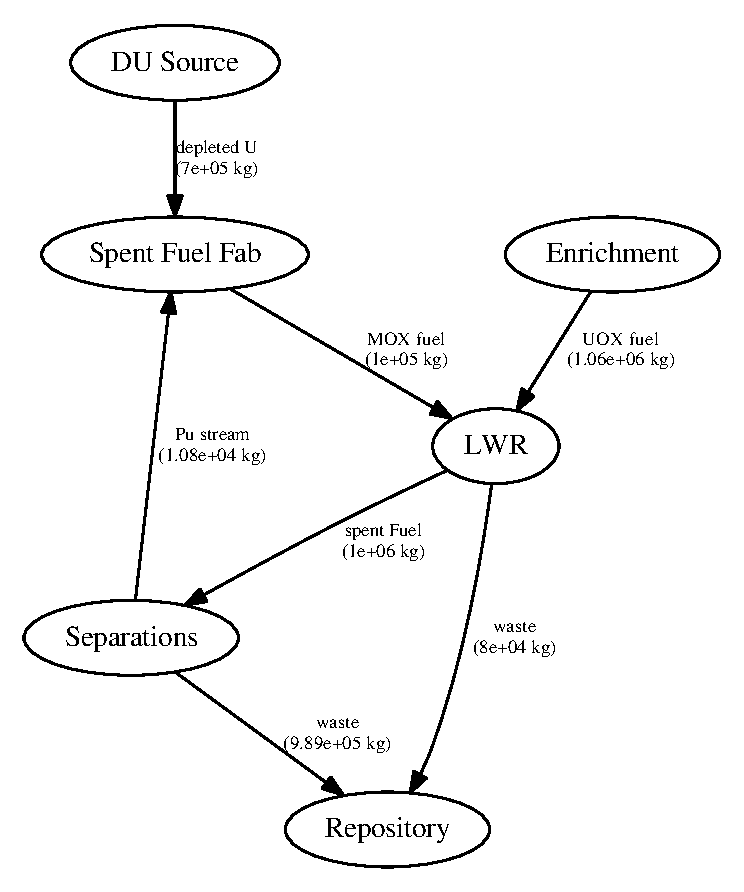
\includegraphics{./images/flow-mod-open-1.eps}
\end{center}
\end{figure}

To switch to a fully closed fuel cycle, all that needs to be done is change
the output commodity for the \textit{BatchReactor}'s spent MOX fuel.  All this
requires is a single word change in the input file resulting in the material
flows in Figure \ref{fig:flow-closed}.  Note that because the
\textit{BatchReactor} always transmutes fuel into the same composition, the
nuclide level flows are not realistic for the full, multipass recycle case.

\TODO{mention how fuel fab mixes fissile and filler streams}

\begin{figure}[!]
\label{fig:flow-closed}
\caption{Full MOX recycle (multi-pass) fuel cycle material flows.}
\begin{center}
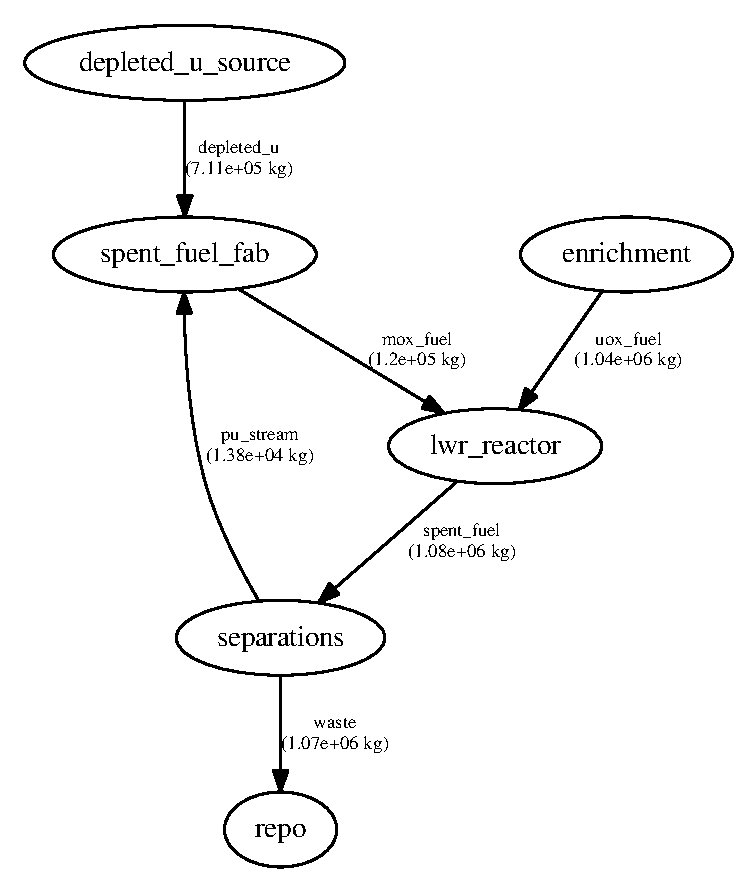
\includegraphics{./images/flow-closed-1.eps}
\end{center}
\end{figure}

\TODO{discuss Pu buildup charts}

\begin{figure}[!]
\label{fig:puseries-1}
\caption{bla}
\begin{center}
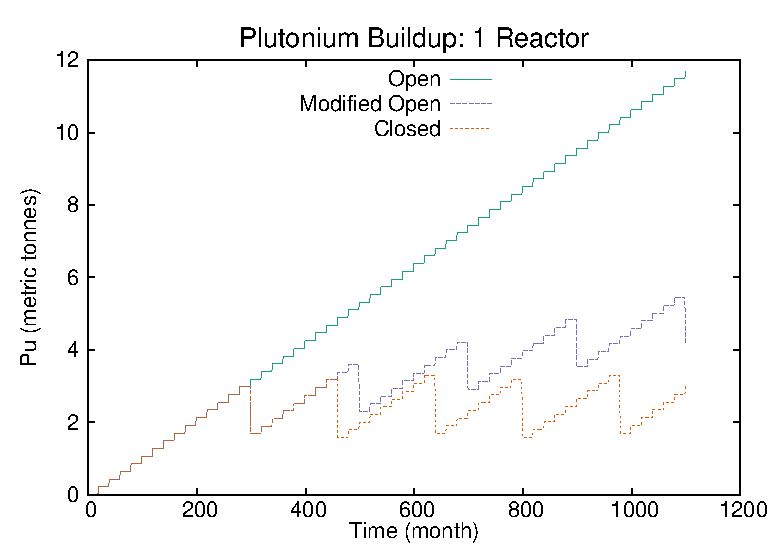
\includegraphics{./images/puseries-1.eps}
\end{center}
\end{figure}

\begin{figure}[!]
\label{fig:puseries-n}
\caption{bla}
\begin{center}
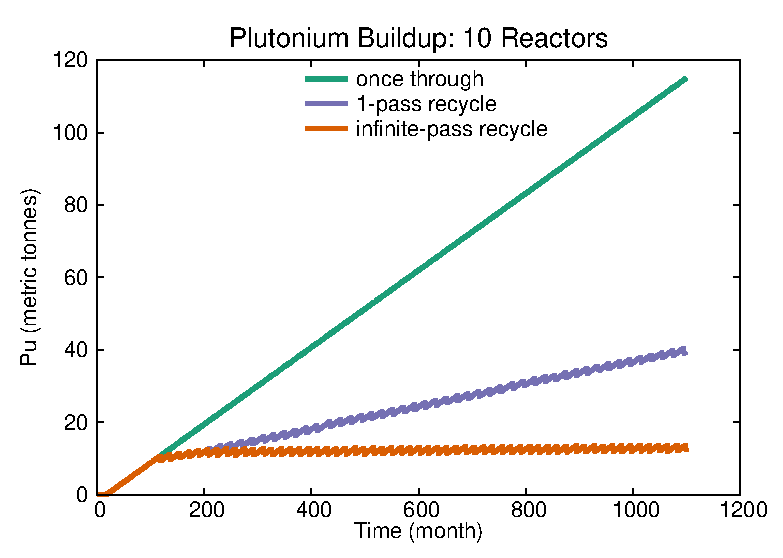
\includegraphics{./images/puseries-n.eps}
\end{center}
\end{figure}

